%%%%%%%%%%%%%%%%%%%%%%%%%%%%%%%%%%%%%%%%%
% Jacobs Landscape Poster
% LaTeX Template
% Version 1.1 (14/06/14)
%
% Created by:
% Computational Physics and Biophysics Group, Jacobs University
% https://teamwork.jacobs-university.de:8443/confluence/display/CoPandBiG/LaTeX+Poster
% 
% Further modified by:
% Nathaniel Johnston (nathaniel@njohnston.ca)
%
% This template has been downloaded from:
% http://www.LaTeXTemplates.com
%
% License:
% CC BY-NC-SA 3.0 (http://creativecommons.org/licenses/by-nc-sa/3.0/)
%
%%%%%%%%%%%%%%%%%%%%%%%%%%%%%%%%%%%%%%%%%

%----------------------------------------------------------------------------------------
%	PACKAGES AND OTHER DOCUMENT CONFIGURATIONS
%----------------------------------------------------------------------------------------

\documentclass[final]{beamer}

\usepackage[scale=1.0]{beamerposter} % Use the beamerposter package for laying out the poster
\usepackage[acronym,toc]{glossaries}
\newacronym[longplural={metric tons of heavy metal}]{MTHM}{MTHM}{metric ton of heavy metal}
\newacronym{ABM}{ABM}{agent-based modeling}
\newacronym{ACDIS}{ACDIS}{Program in Arms Control \& Domestic and International Security}
\newacronym{AHTR}{AHTR}{Advanced High Temperature Reactor}
\newacronym{ANDRA}{ANDRA}{Agence Nationale pour la gestion des D\'echets RAdioactifs, the French National Agency for Radioactive Waste Management}
\newacronym{ANL}{ANL}{Argonne National Laboratory}
\newacronym{API}{API}{application programming interface}
\newacronym{ARCH}{ARCH}{autoregressive conditional heteroskedastic}
\newacronym{ARE}{ARE}{Aircraft Reactor Experiment}
\newacronym{ARFC}{ARFC}{Advanced Reactors and Fuel Cycles}
\newacronym{ARMA}{ARMA}{autoregressive moving average}
\newacronym{ASME}{ASME}{American Society of Mechanical Engineers}
\newacronym{ATWS}{ATWS}{Anticipated Transient Without Scram}
\newacronym{BDBE}{BDBE}{Beyond Design Basis Event}
\newacronym{BIDS}{BIDS}{Berkeley Institute for Data Science}
\newacronym{BOL}{BOL}{Beginning-of-Life}
\newacronym{BSD}{BSD}{Berkeley Software Distribution}
\newacronym{CAFCA}{CAFCA}{ Code for Advanced Fuel Cycles Assessment }
\newacronym{CASL}{CASL}{Consortium for Advanced Simulation of Light Water Reactors}
\newacronym{CDTN}{CDTN}{Centro de Desenvolvimento da Tecnologia Nuclear}
\newacronym{CEA}{CEA}{Commissariat \`a l'\'Energie Atomique et aux \'Energies Alternatives}
\newacronym{CI}{CI}{continuous integration}
\newacronym{CNEC}{CNEC}{Consortium for Nonproliferation Enabling Capabilities}
\newacronym{CNEN}{CNEN}{Comiss\~{a}o Nacional de Energia Nuclear}
\newacronym{CNERG}{CNERG}{Computational Nuclear Engineering Research Group}
\newacronym{COSI}{COSI}{Commelini-Sicard}
\newacronym{COTS}{COTS}{commercial, off-the-shelf}
\newacronym{CSNF}{CSNF}{commercial spent nuclear fuel}
\newacronym{CTAH}{CTAHs}{Coiled Tube Air Heaters}
\newacronym{CUBIT}{CUBIT}{CUBIT Geometry and Mesh Generation Toolkit}
\newacronym{CURIE}{CURIE}{Centralized Used Fuel Resource for Information Exchange}
\newacronym{DAG}{DAG}{directed acyclic graph}
\newacronym{DANESS}{DANESS}{Dynamic Analysis of Nuclear Energy System Strategies}
\newacronym{DBE}{DBE}{Design Basis Event}
\newacronym{DESAE}{DESAE}{Dynamic Analysis of Nuclear Energy Systems Strategies}
\newacronym{DHS}{DHS}{Department of Homeland Security}
\newacronym{DOE}{DOE}{Department of Energy}
\newacronym{DRACS}{DRACS}{Direct Reactor Auxiliary Cooling System}
\newacronym{DRE}{DRE}{dynamic resource exchange}
\newacronym{DSNF}{DSNF}{DOE spent nuclear fuel}
\newacronym{DYMOND}{DYMOND}{Dynamic Model of Nuclear Development }
\newacronym{EBS}{EBS}{Engineered Barrier System}
\newacronym{EDZ}{EDZ}{Excavation Disturbed Zone}
\newacronym{EIA}{EIA}{U.S. Energy Information Administration}
\newacronym{EPA}{EPA}{Environmental Protection Agency}
\newacronym{EP}{EP}{Engineering Physics}
\newacronym{FCO}{FCO}{Fuel Cycle Options}
\newacronym{FCT}{FCT}{Fuel Cycle Technology}
\newacronym{FCWMD}{FCWMD}{Fuel Cycle and Waste Management Division}
\newacronym{FEHM}{FEHM}{Finite Element Heat and Mass Transfer}
\newacronym{FEPs}{FEPs}{Features, Events, and Processes}
\newacronym{FHR}{FHR}{Fluoride-Salt-Cooled High-Temperature Reactor}
\newacronym{FLiBe}{FLiBe}{Fluoride-Lithium-Beryllium}
\newacronym{GCAM}{GCAM}{Global Change Assessment Model}
\newacronym{GDSE}{GDSE}{Generic Disposal System Environment}
\newacronym{GDSM}{GDSM}{Generic Disposal System Model}
\newacronym{GENIUSv1}{GENIUSv1}{Global Evaluation of Nuclear Infrastructure Utilization Scenarios, Version 1}
\newacronym{GENIUSv2}{GENIUSv2}{Global Evaluation of Nuclear Infrastructure Utilization Scenarios, Version 2}
\newacronym{GENIUS}{GENIUS}{Global Evaluation of Nuclear Infrastructure Utilization Scenarios}
\newacronym{GPAM}{GPAM}{Generic Performance Assessment Model}
\newacronym{GRSAC}{GRSAC}{Graphite Reactor Severe Accident Code}
\newacronym{GUI}{GUI}{graphical user interface}
\newacronym{HLW}{HLW}{high level waste}
\newacronym{HPC}{HPC}{high-performance computing}
\newacronym{HTC}{HTC}{high-throughput computing}
\newacronym{HTGR}{HTGR}{High Temperature Gas-Cooled Reactor}
\newacronym{IAEA}{IAEA}{International Atomic Energy Agency}
\newacronym{IEMA}{IEMA}{Illinois Emergency Mangament Agency}
\newacronym{INL}{INL}{Idaho National Laboratory}
\newacronym{IPRR1}{IRP-R1}{Instituto de Pesquisas Radioativas Reator 1}
\newacronym{IRP}{IRP}{Integrated Research Project}
\newacronym{ISFSI}{ISFSI}{Independent Spent Fuel Storage Installation}
\newacronym{ISRG}{ISRG}{Independent Student Research Group}
\newacronym{JFNK}{JFNK}{Jacobian-Free Newton Krylov}
\newacronym{LANL}{LANL}{Los Alamos National Laboratory}
\newacronym{LBNL}{LBNL}{Lawrence Berkeley National Laboratory}
\newacronym{LCOE}{LCOE}{levelized cost of electricity}
\newacronym{LDRD}{LDRD}{laboratory directed research and development}
\newacronym{LFR}{LFR}{Lead-Cooled Fast Reactor}
\newacronym{LGPL}{LGPL}{Lesser GNU Public License}
\newacronym{LLNL}{LLNL}{Lawrence Livermore National Laboratory}
\newacronym{LMFBR}{LMFBR}{Liquid-Metal-cooled Fast Breeder Reactor}
\newacronym{LOFC}{LOFC}{Loss of Forced Cooling}
\newacronym{LOHS}{LOHS}{Loss of Heat Sink}
\newacronym{LOLA}{LOLA}{Loss of Large Area}
\newacronym{LP}{LP}{linear program}
\newacronym{LWR}{LWR}{Light Water Reactor}
\newacronym{MARKAL}{MARKAL}{MARKet and ALlocation}
\newacronym{MA}{MA}{minor actinide}
\newacronym{MCNP}{MCNP}{Monte Carlo N-Particle code}
\newacronym{MILP}{MILP}{mixed-integer linear program}
\newacronym{MIT}{MIT}{the Massachusetts Institute of Technology}
\newacronym{MOAB}{MOAB}{Mesh-Oriented datABase}
\newacronym{MOOSE}{MOOSE}{Multiphysics Object-Oriented Simulation Environment}
\newacronym{MOX}{MOX}{mixed oxide}
\newacronym{MSBR}{MSBR}{Molten Salt Breeder Reactor}
\newacronym{MSRE}{MSRE}{Molten Salt Reactor Experiment}
\newacronym{MSR}{MSR}{Molten Salt Reactor}
\newacronym{NAGRA}{NAGRA}{National Cooperative for the Disposal of Radioactive Waste}
\newacronym{NCSA}{NCSA}{National Center for Supercomputing Applications}
\newacronym{NEAMS}{NEAMS}{Nuclear Engineering Advanced Modeling and Simulation}
\newacronym{NEUP}{NEUP}{Nuclear Energy University Programs}
\newacronym{NFCSim}{NFCSim}{Nuclear Fuel Cycle Simulator}
\newacronym{NFC}{NFC}{Nuclear Fuel Cycle}
\newacronym{NGNP}{NGNP}{Next Generation Nuclear Plant}
\newacronym{NMWPC}{NMWPC}{Nuclear MW Per Capita}
\newacronym{NNSA}{NNSA}{National Nuclear Security Administration}
\newacronym{NPRE}{NPRE}{Department of Nuclear, Plasma, and Radiological Engineering}
\newacronym{NQA1}{NQA-1}{Nuclear Quality Assurance - 1}
\newacronym{NRC}{NRC}{Nuclear Regulatory Commission}
\newacronym{NSF}{NSF}{National Science Foundation}
\newacronym{NSSC}{NSSC}{Nuclear Science and Security Consortium}
\newacronym{NUWASTE}{NUWASTE}{Nuclear Waste Assessment System for Technical Evaluation}
\newacronym{NWF}{NWF}{Nuclear Waste Fund}
\newacronym{NWTRB}{NWTRB}{Nuclear Waste Technical Review Board}
\newacronym{OCRWM}{OCRWM}{Office of Civilian Radioactive Waste Management}
\newacronym{ORION}{ORION}{ORION}
\newacronym{ORNL}{ORNL}{Oak Ridge National Laboratory}
\newacronym{PARCS}{PARCS}{Purdue Advanced Reactor Core Simulator}
\newacronym{PBAHTR}{PB-AHTR}{Pebble Bed Advanced High Temperature Reactor}
\newacronym{PBFHR}{PB-FHR}{Pebble-Bed Fluoride-Salt-Cooled High-Temperature Reactor}
\newacronym{PEI}{PEI}{Peak Environmental Impact}
\newacronym{PH}{PRONGHORN}{PRONGHORN}
\newacronym{PI}{PI}{Principal Investigator}
\newacronym{PNNL}{PNNL}{Pacific Northwest National Laboratory}
\newacronym{PRIS}{PRIS}{Power Reactor Information System}
\newacronym{PRKE}{PRKE}{Point Reactor Kinetics Equations}
\newacronym{PSPG}{PSPG}{Pressure-Stabilizing/Petrov-Galerkin}
\newacronym{PWAR}{PWAR}{Pratt and Whitney Aircraft Reactor}
\newacronym{PWR}{PWR}{Pressurized Water Reactor}
\newacronym{PyNE}{PyNE}{Python toolkit for Nuclear Engineering}
\newacronym{PyRK}{PyRK}{Python for Reactor Kinetics}
\newacronym{QA}{QA}{quality assurance}
\newacronym{RDD}{RD\&D}{Research Development and Demonstration}
\newacronym{RD}{R\&D}{Research and Development}
\newacronym{RELAP}{RELAP}{Reactor Excursion and Leak Analysis Program}
\newacronym{RIA}{RIA}{Reactivity Insertion Accident}
\newacronym{RIF}{RIF}{Region-Institution-Facility}
\newacronym{SAM}{SAM}{Simulation and Modeling}
\newacronym{SCF}{SCF}{Software Carpentry Foundation}
\newacronym{SFR}{SFR}{Sodium-Cooled Fast Reactor}
\newacronym{SINDAG}{SINDA{\textbackslash}G}{Systems Improved Numerical Differencing Analyzer $\backslash$ Gaski}
\newacronym{SKB}{SKB}{Svensk K\"{a}rnbr\"{a}nslehantering AB}
\newacronym{SNF}{SNF}{spent nuclear fuel}
\newacronym{SNL}{SNL}{Sandia National Laboratory}
\newacronym{SNM}{SNM}{Special Nuclear Material}
\newacronym{STC}{STC}{specific temperature change}
\newacronym{SUPG}{SUPG}{Streamline-Upwind/Petrov-Galerkin}
\newacronym{SWF}{SWF}{Separations and Waste Forms}
\newacronym{SWU}{SWU}{Separative Work Unit}
\newacronym{SandO}{S\&O}{Signatures and Observables}
\newacronym{THW}{THW}{The Hacker Within}
\newacronym{TRIGA}{TRIGA}{Training Research Isotope General Atomic}
\newacronym{TRISO}{TRISO}{Tristructural Isotropic}
\newacronym{TSM}{TSM}{Total System Model}
\newacronym{TSPA}{TSPA}{Total System Performance Assessment for the Yucca Mountain License Application}
\newacronym{UDB}{UDB}{Unified Database}
\newacronym{UFD}{UFD}{Used Fuel Disposition}
\newacronym{UML}{UML}{Unified Modeling Language}
\newacronym{UNFSTANDARDS}{UNFST\&DARDS}{Used Nuclear Fuel Storage, Transportation \& Disposal Analysis Resource and Data System}
\newacronym{UOX}{UOX}{uranium oxide}
\newacronym{UQ}{UQ}{uncertainty quantification}
\newacronym{US}{US}{United States}
\newacronym{UW}{UW}{University of Wisconsin}
\newacronym{VISION}{VISION}{the Verifiable Fuel Cycle Simulation Model}
\newacronym{VV}{V\&V}{verification and validation}
\newacronym{WIPP}{WIPP}{Waste Isolation Pilot Plant}
\newacronym{YMG}{YMG}{Young Members Group}
\newacronym{YMR}{YMR}{Yucca Mountain Repository Site}
\newacronym{NEI}{NEI}{Nuclear Energy Institute}
%\newacronym{<++>}{<++>}{<++>}
%\newacronym{<++>}{<++>}{<++>}

\usetheme{confposter} % Use the confposter theme supplied with this template

\setbeamercolor{block title}{fg=dblue!80,bg=white} % Colors of the block titles
\setbeamercolor{block body}{fg=black,bg=white} % Colors of the body of blocks
\setbeamercolor{block alerted title}{fg=white,bg=dblue!70} % Colors of the highlighted block titles
\setbeamercolor{block alerted body}{fg=black,bg=dblue!10} % Colors of the body of highlighted blocks
% Many more colors are available for use in beamerthemeconfposter.sty

%-----------------------------------------------------------
% Define the column widths and overall poster size
% To set effective sepwid, onecolwid and twocolwid values, first choose how many columns you want and how much separation you want between columns
% In this template, the separation width chosen is 0.024 of the paper width and a 4-column layout
% onecolwid should therefore be (1-(# of columns+1)*sepwid)/# of columns e.g. (1-(4+1)*0.024)/4 = 0.22
% onecolwid should therefore be (1-(# of columns+1)*sepwid)/# of columns e.g. 
% (1-(3+1)*0.025)/3 = 0.3
% Set twocolwid to be (2*onecolwid)+sepwid = 0.464
% Set threecolwid to be (3*onecolwid)+2*sepwid = 0.708

\newlength{\sepwid}
\newlength{\onecolwid}
\newlength{\twocolwid}
\newlength{\threecolwid}
\setlength{\paperwidth}{36in} % A0 width: 46.8in
\setlength{\paperheight}{48in} % A0 height: 33.1in
\setlength{\textwidth}{34in} % A0 width: 46.8in
\setlength{\textheight}{46in} % A0 height: 33.1in
\setlength{\sepwid}{0.025\paperwidth} % Separation width (white space) between columns
\setlength{\onecolwid}{0.3\paperwidth} % Width of one column
\setlength{\twocolwid}{0.625\paperwidth} % Width of two columns
\setlength{\threecolwid}{0.95\paperwidth} % Width of three columns
\setlength{\topmargin}{-0.5in} % Reduce the top margin size
%-----------------------------------------------------------

\usepackage{graphicx}  % Required for including images
\newcommand{\Cyclus}{\textsc{Cyclus}\xspace}%
\usepackage{tabularx}
\newcolumntype{b}{X}
\newcolumntype{s}{>{\hsize=.5\hsize}X}
\newcolumntype{m}{>{\hsize=.75\hsize}X}
\newcolumntype{z}{>{\hsize=.65\hsize}X}

\usepackage{booktabs} % Top and bottom rules for tables
\usepackage{xspace}
\usepackage{amsmath}
\usepackage{exscale}
\usepackage[labelformat=simple]{caption}


\setbeamertemplate{bibliography item}[text]




%----------------------------------------------------------------------------------------
%	TITLE SECTION 
%----------------------------------------------------------------------------------------

\title{%
  \texorpdfstring{%
    \makebox[\linewidth]{%
      \makebox[0pt][l]{%
        \raisebox{\dimexpr-\height+\baselineskip}[0pt][0pt]
          {
\includegraphics[height=2.5\baselineskip]{UIUC_Logo}}% Left logo
      }\hfill
      \makebox[0pt]{Comparison Between Continuous and Batchwise}%
      \hfill\makebox[0pt][r]{%
        \raisebox{\dimexpr-\height+\baselineskip}[0pt][0pt]
          {
\includegraphics[height=3.3\baselineskip]{arfc_atom}}% Right logo
      }%
    }%
  }
  % To make a title with two lines, remove the "%" from the following two lines 
  {Comparison Between Continuous and Batchwise}
  {Online Reprocessing in Serpent2}
  {\vspace{1cm}}
  } % Poster title

\author{\textbf{Luke Seifert}, Madicken Munk}
\institute{University of Illinios at Urbana-Champaign, Department of Nuclear, Plasma, and Radiological Engineering, Urbana, IL 61801}
%----------------------------------------------------------------------------------------

\begin{document}

\addtobeamertemplate{block end}{}{\vspace*{2ex}} % White space under blocks
\addtobeamertemplate{block alerted end}{}{\vspace*{2ex}} % White space under highlighted (alert) blocks

\setlength{\belowcaptionskip}{2ex} % White space under figures
\setlength\belowdisplayshortskip{2ex} % White space under equations

\begin{frame}[t] % The whole poster is enclosed in one beamer frame

\begin{columns}[t,totalwidth=\threecolwid] % The whole poster consists of three major columns, the second of which is split into two columns twice - the [t] option aligns each column's content to the top

\begin{column}{0.5\sepwid}\end{column} % Empty spacer column

\begin{column}{\onecolwid} % The first column

%----------------------------------------------------------------------------------------
%	INTRODUCTION
%----------------------------------------------------------------------------------------

\begin{block}{Introduction}

\textbf{Molten Salt Reactor Online Reprocessing}

\begin{itemize}
	\item Depletion of a reactor provides useful data on safety parameter and fuel cycle evolution
	\item Depletion of Molten Salt Reactors requires accounting for reprocessing
	\item Batchwise modeling of Molten Salt Reactors is common \cite{rykhlevskii_modeling_2019, betzler_molten_2017}
	\item Continuous modeling offers unique advantages over batchwise modeling
\end{itemize}

\vspace{0.7em}
\textbf{Comparison of Methods}

\begin{itemize}
	\item An identical toy model is implemented for both methods
	\item Continuous model uses varying number of steps
	\item Multiple approaches are implemented for the continuous model
	%\item Potential weaknesses of continuous model are investigated
\end{itemize}


\begin{figure}
	\label{fig:toy_geom}
	
\includegraphics[width=0.6\linewidth]{images/CR0_geom1.png}
	\caption{Geometry of toy model used in serpent2 for continuous and batchwise reprocessing models. Composed of a cube of fuel salt with a graphite log in the center and a graphite shell.}
\end{figure}



\begin{table}[H]
\renewcommand{\arraystretch}{1.25}
\caption{Approach Acronyms and Descriptions}
\label{tab:res_key}
\begin{center}
\begin{tabular}{ | c | c | }
 \hline
        Approach & Description\\
 \hline
 \hline
 	SP pre & SaltProc steady batch pre-depletion\\
	SP post & SaltProc steady batch post-depletion\\
	CR & Cycle Rate continuous approach\\
	SPCR & SaltProc Cycle Rate continuous approach\\
	CTD & Cycle Time Decay continuous approach\\
	CTRL & Control method (no reprocessing feeds or removal)\\
 \hline
\end{tabular}
\end{center}
\end{table}

\end{block}

%----------------------------------------------------------------------------------------
%	OBJECTIVES
%----------------------------------------------------------------------------------------

%This section creates an orange border around a white box
\setbeamercolor{block alerted title}{fg=black,bg=norange} % Change the alert block title colors
\setbeamercolor{block alerted body}{fg=black,bg=white} % Change the alert block body colors
\begin{alertblock}{Objectives}
\begin{itemize}
        \item Capture the precise differences in continuous and batchwise models
	\item Determine effective depletion step sizes for continuous reprocessing
	\item Investigate validity of using average feed rates during depletion
	%\item Investigate potential weaknesses of continuous reprocessing
\end{itemize}

\end{alertblock}



\setbeamercolor{block alerted title}{fg=white,bg=dblue} % Change the alert block title colors
\setbeamercolor{block alerted body}{fg=black,bg=white} % Change the alert block body colors

\begin{alertblock}{Contact Information}
	\setbeamercolor{block title}{fg=norange,bg=white} % Change the block title color
	\begin{itemize}
		\item Email: \href{mailto:seifert5@illinois.edu}{seifert5@illinois.edu}
		\item Phone: \href{tel:18652790603}{+1 865 279 0603}
	\end{itemize}
% These specific elements are optional, but you should have some method for people to contact you.	
	
\end{alertblock}





%----------------------------------------------------------------------------------------
%	Programs
%----------------------------------------------------------------------------------------

%\begin{block}{Program 1}
%Description
%
%\begin{figure}
%	\label{fig:figure_label_ex1}
%	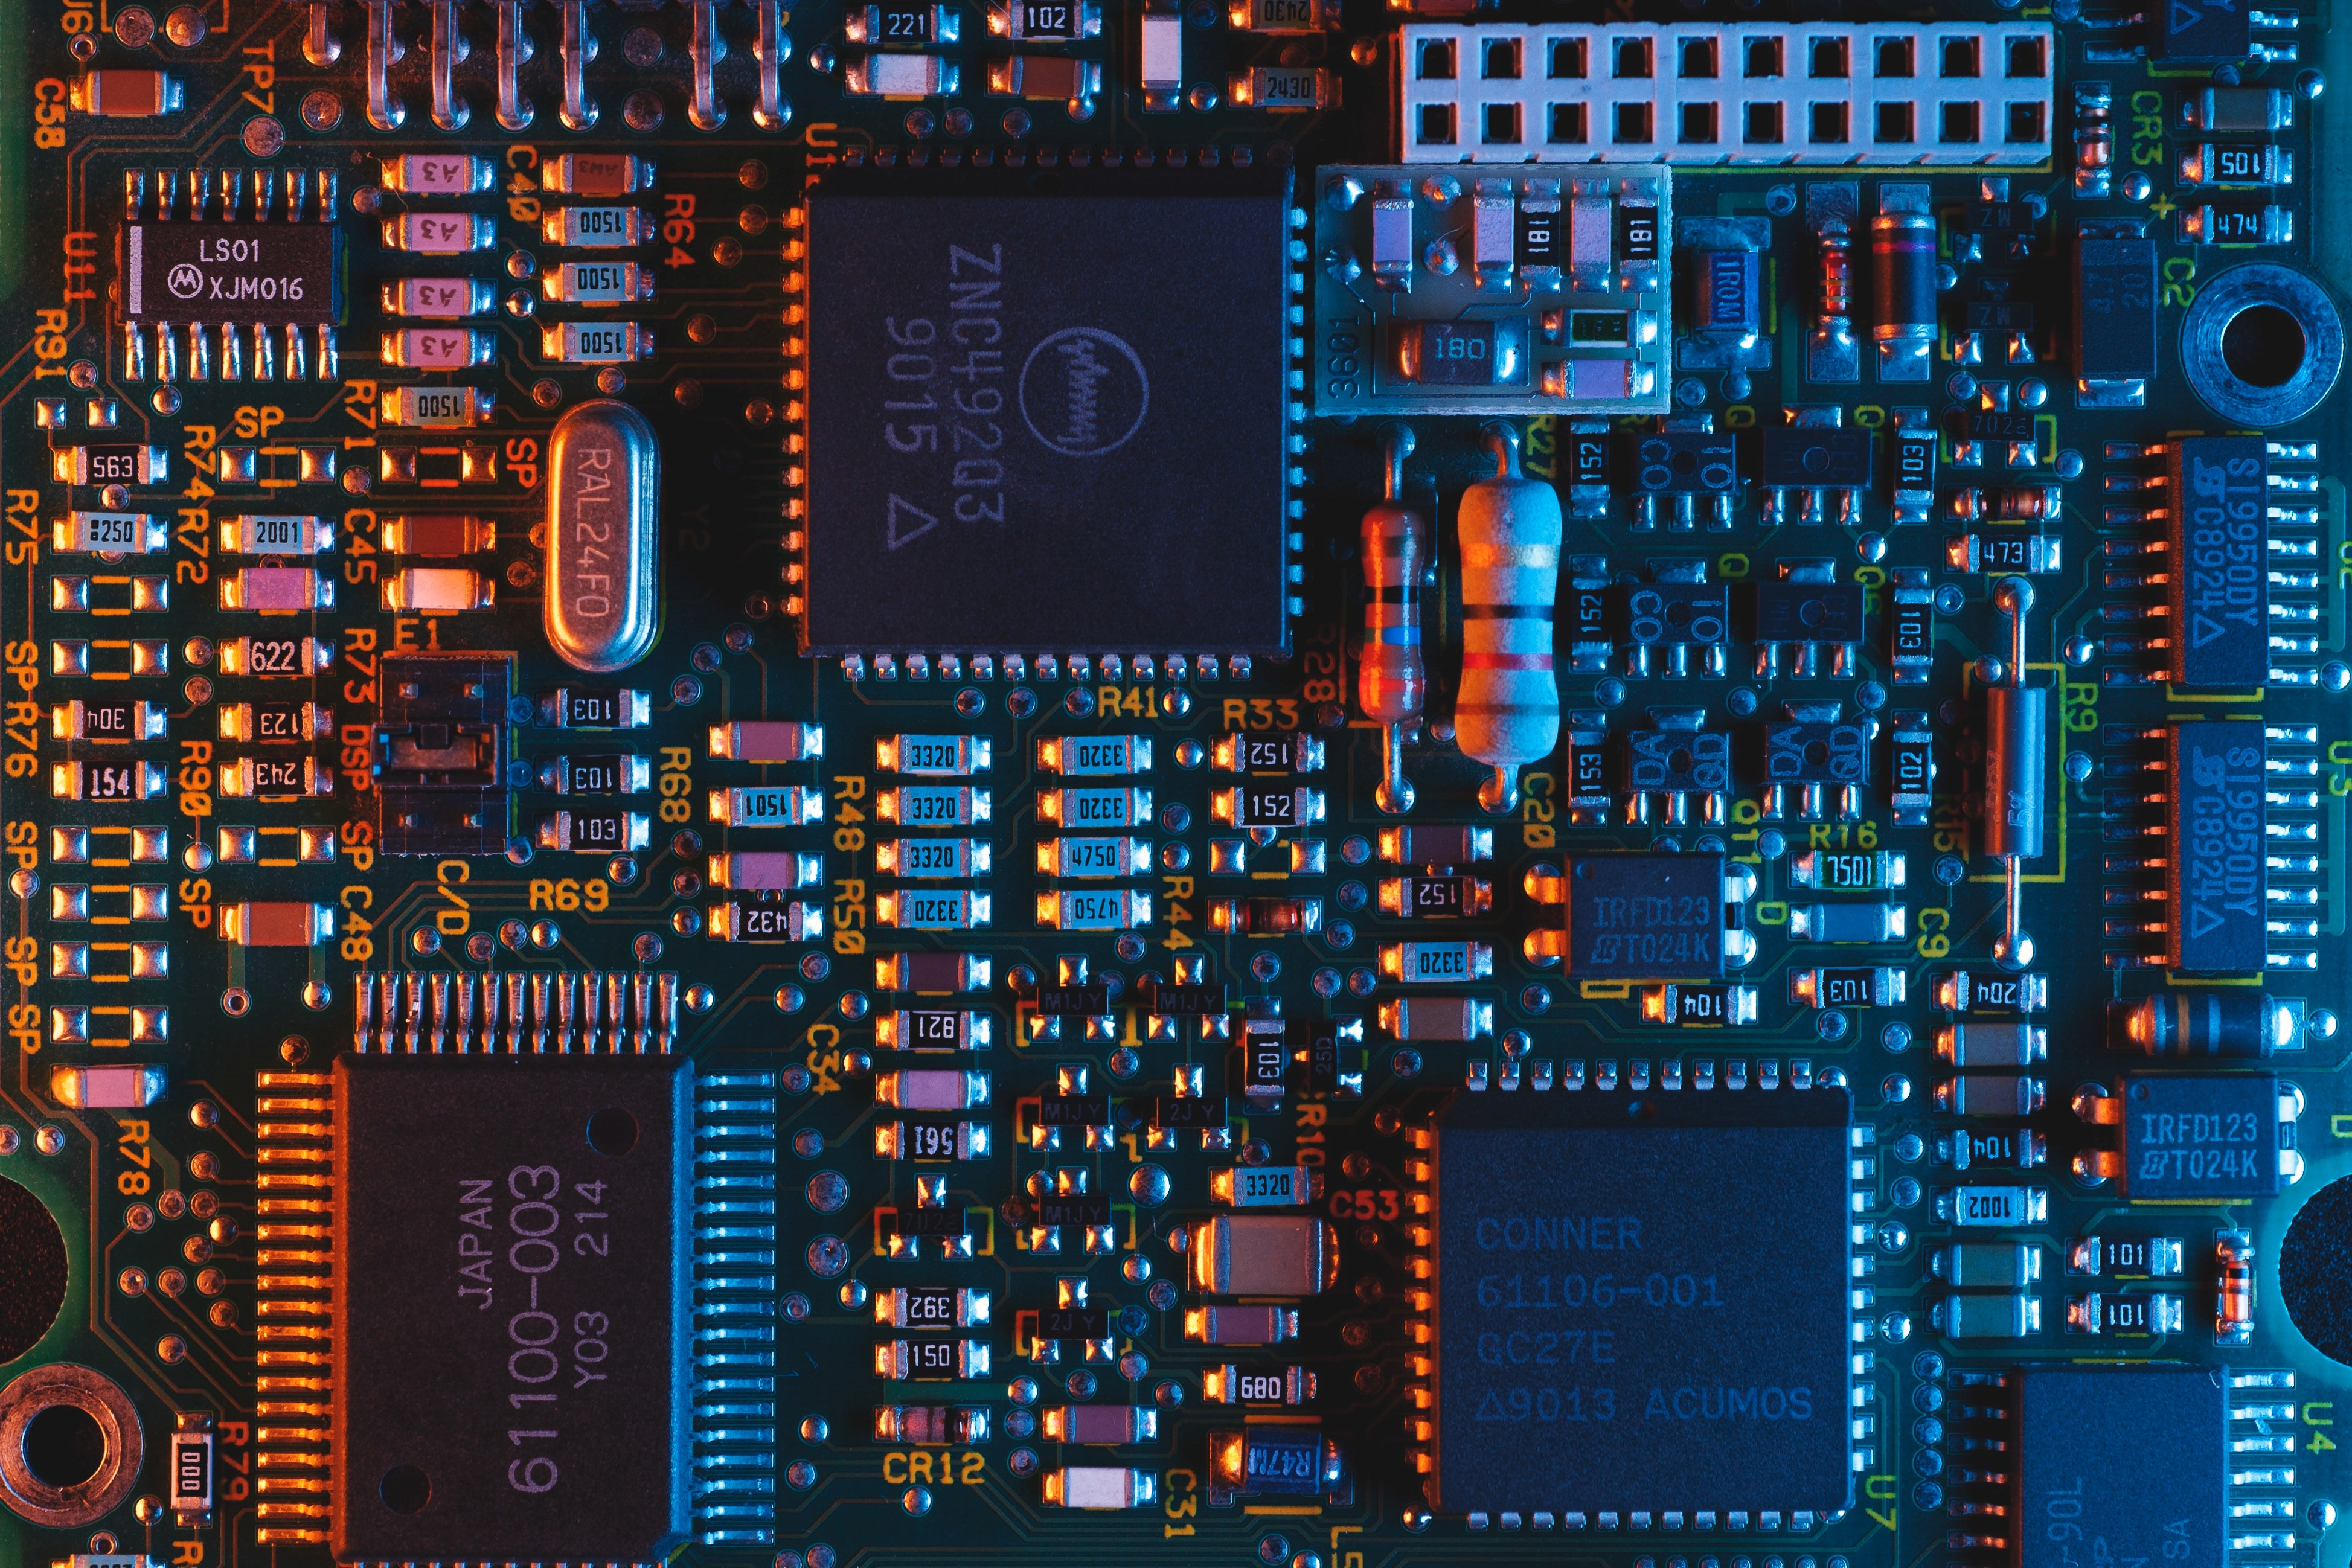
\includegraphics[width=0.9\linewidth]{graphic_name1}
%	\caption{Caption1 Reference \cite{call_tag_article}}
%\end{figure}
%
%\end{block}
%
%\begin{block}{Program 2}
%
%Description
% 
%\begin{itemize}
%	\item{Item 1}
%	\item{Item 2}
%	\item{Item 3}
%\end{itemize}
%
%\end{block}
%
%----------------------------------------------------------------------------------------

\end{column} % End of the first column

\begin{column}{\sepwid}\end{column} % Empty spacer column


%----------------------------------------------------------------------------------------

\begin{column}{\onecolwid} % The second column
%----------------------------------------------------------------------------------------
%	MODELS
%----------------------------------------------------------------------------------------

\begin{block}{Reprocessing Models}
\vspace{0.7em}
\textbf{Batchwise Reprocessing}

\begin{itemize}
        \item Iteratively perform depletion with external adjustments
	\item \textbf{\emph{Steady Batch}} uses small removals each depletion step.

\begin{align}
	X = \frac{1}{T_{cyc}}
\end{align}
	\begin{itemize}
		\item $T_{cyc}$ is the cycle time
		\item $X$ is the fractional removal rate
	\end{itemize}

	%\item Small removals each depletion step is Steady Batch
	\item \textbf{\emph{Bulk Batch}} uses full removal after a set number of depletion steps.
	%\item Full removal after set number of steps is Bulk Batch
	\item SaltProc is used to run batchwise reprocessing for Serpent2
	\item The current version of SaltProc uses the Steady Batch method
\end{itemize}


\begin{table}[H]
\renewcommand{\arraystretch}{1.25}
\caption{Batchwise Reprocessing Methods}
\label{tab:batch_methods}
\begin{center}
\begin{tabular}{ | c | c | c | c | }
 \hline
	Approach & Cycle Time & X [s$^{-1}$] & Step Removal\\
 \hline
 \hline
	Bulk Batch [3d] & 20 s & - & 1\\
	Bulk Batch [3d] & 30 d & - & \, 0$^{*}$ \\
	Steady Batch [3d] & 20 s & 3.86E-6 & 1\\
	Steady Batch [3d] & 3 d & 3.86E-6 & 1\\
	Steady Batch [3d] & 30 d & 3.86E-7 & 0.1\\
 \hline
\end{tabular}
\end{center}
\end{table}
	\begin{center}
\footnotesize{$^{*}$ Bulk removal occurs after 30 days, so the step fractional removal becomes 1 at 30 day step.}\\
	\end{center}

\vspace{0.7em}
\textbf{Continuous Reprocessing}

\begin{itemize}
	\item Adds "decay-like" term to Bateman equation, less iterative \cite{aufiero_extended_2013}

%\begin{align}
%\frac{dN_j}{dt}_{base} = \sum_{i \neq j}  \left [ \left( \gamma_{i \rightarrow j} \sigma_{f, i} \Phi + \lambda _{i \rightarrow j} + \sigma_{i \rightarrow j} \Phi \right) N_i \right ] - \left ( \lambda_j + \sigma_j \Phi \right ) N_j
%\end{align}

\begin{equation} \hfill
\begin{split}
%\frac{dN}{dt} = \sum_j \lambda_j N_j + \gamma \Sigma_f \phi + \Sigma_k \phi - \lambda N - \Sigma \phi - C
\frac{dN_j}{dt}_{base} = \sum_{i \neq j}  & \left [ \left( \gamma_{i \rightarrow j} \sigma_{f, i} \Phi + \lambda _{i \rightarrow j} + \sigma_{i \rightarrow j} \Phi \right) N_i \right ]\\
 & - \left ( \lambda_j + \sigma_j \Phi \right ) N_j
\end{split}
\hfill\label{eq:Bateman_default} \end{equation}




\begin{align}	
\frac{dN_j}{dt}_{net} = \frac{dN_j}{dt}_{base} -  \lambda_{r, j} N_j + \sum_{mat} \lambda _{r, i \rightarrow j} N_i
\end{align}


The symbols given in the equations are defined as follows:
\begin{itemize}
\item $N_j$ is the atomic density of isotope j.
\item $\gamma_{i \rightarrow j}$ is the fractional fission product yield of $j$ in the fission of isotope $i$.
\item $\sigma_{f, i}$ is the microscopic fission cross section of isotope $i$.
\item $\Phi$ is the spectrum-averaged scalar flux in the fuel region.
\item $\lambda _{i \rightarrow j}$ is the decay constant of decay $i \rightarrow j$.
\item $\sigma_{i \rightarrow j}$ is the microscopic transmution cross section of reaction $i \rightarrow j$.
\item $N_i$ is the atomic density of isotope $i$.
\item $\lambda_j$ is the decay constant of isotope $j$.
\item $\lambda_{r, j}$ is the reprocessing constant for removal of isotope $j$.
\item $\sigma_j$ is the microscopic total transmutation cross section of isotope $j$.
\item $\lambda _{r, i \rightarrow j}$ is the reprocessing constant for feed of material $i \rightarrow j$.
\end{itemize}


	\item \textbf{\emph{Cycle Time Decay}} (CTD) model treats reprocessing as decay


\begin{align}
	\tau_{1/2} = \frac{1}{2} T_{cyc}
\end{align}

\begin{align}
	\lambda_r = \frac{ln(2)}{\tau_{1/2}}
\end{align}

	\item \textbf{\emph{Cycle Rate}} (CR) treats as linear fractional removal, same as Steady Batch

\begin{align}
	\lambda_r = ln \left( \frac{1}{1-X} \right)
\end{align}


	\item \textbf{\emph{SaltProc Cycle Rate}} (SPCR) mimics batchwise reprocessing with continuous model
\end{itemize}


\begin{table}[H]
\renewcommand{\arraystretch}{1.25}
\caption{Continuous Reprocessing Methods}
\label{tab:cont_methods}
\begin{center}
\begin{tabular}{ | c | c | c | c | c | }
 \hline
	Approach & Cycle Time & $\tau_{1/2}$ & X [s$^{-1}$] & $\lambda_{r}$ [s$^{-1}$]\\
 \hline
 \hline
 Cycle Time Decay & 20 s & 10 s & 6.70E-2 & 6.93E-2\\
 Cycle Time Decay & 3 d & 1.5 d & 5.35E-6 & 5.35E-6\\
 Cycle Rate & 20 s & - & 0.05 & 5.13E-2\\
 Cycle Rate & 3 d & - & 3.86E-6 & 3.86E-6\\
 SaltProc Cycle Rate & 20 s & - & 3.86E-6 & 3.86E-6\\
 SaltProc Cycle Rate & 3 d & - & 3.86E-6 & 3.86E-6\\
 SaltProc Cycle Rate & 30 d & - & 3.86E-7 & 3.86E-7\\
 
 \hline
\end{tabular}
\end{center}
\end{table}



%\vspace{0.7em}
%\textbf{Model Overview}
%
%\begin{table}[H]
%\renewcommand{\arraystretch}{1.25}
%\caption{Different Reprocessing Approaches}
%\label{tab:keff_vals}
%\begin{center}
%\begin{tabular}{ | c | c | c | c | c | }
% \hline
%	Approach & Cycle Time & $\tau_{1/2}$ & X [s$^{-1}$] & $\lambda_{r}$ [s$^{-1}$]\\
% \hline
% \hline
% Bulk Batch [3d] & 20 s & - & - & -\\
% Bulk Batch [3d] & 30 d & - & - & -\\
% Steady Batch [3d] & 20 s & - & 3.86E-6 & -\\
% Steady Batch [3d] & 3 d & - & 3.86E-6 & -\\
% Steady Batch [3d] & 30 d & - & 3.86E-7 & -\\
% \hline
% Cycle Time Decay & 20 s & 10 s & - & 6.93E-2\\
% Cycle Time Decay & 3 d & 1.5 d & - & 5.35E-6\\
% Cycle Rate & 20 s & - & 0.05 & 5.13E-2\\
% Cycle Rate & 3 d & - & 3.86E-6 & 3.86E-6\\
% SaltProc Cycle Rate & 20 s & - & 3.86E-6 & 3.86E-6\\
% SaltProc Cycle Rate & 3 d & - & 3.86E-6 & 3.86E-6\\
% SaltProc Cycle Rate & 30 d & - & 3.86E-7 & 3.86E-7\\
% 
% \hline
%\end{tabular}
%\end{center}
%\end{table}


\end{block}

%----------------------------------------------------------------------------------------

\end{column} % End of column 2

\begin{column}{\sepwid}\end{column} % Empty spacer column

\begin{column}{\onecolwid} % The third column

\begin{block}{Results}
%\textbf{Mass Balancing}
%
%\begin{figure}
%	\label{fig:mass_bal}
%	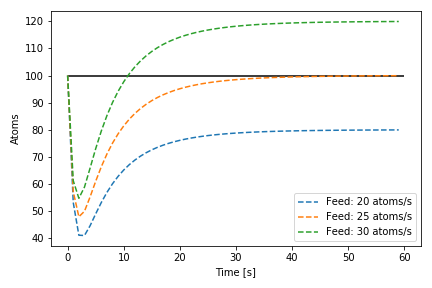
\includegraphics[width=0.9\linewidth]{images/simple_mass_bal.png}
%	\caption{Continuous reprocessing mass balance for single fissile feed and two isotope system with $\tau_{1/2}$ of 10 seconds.}
%\end{figure}
%
%\vspace{0.7em}
%\textbf{Comparison Results}

%\begin{figure}
%	\label{fig:keff_30d_batch}
%	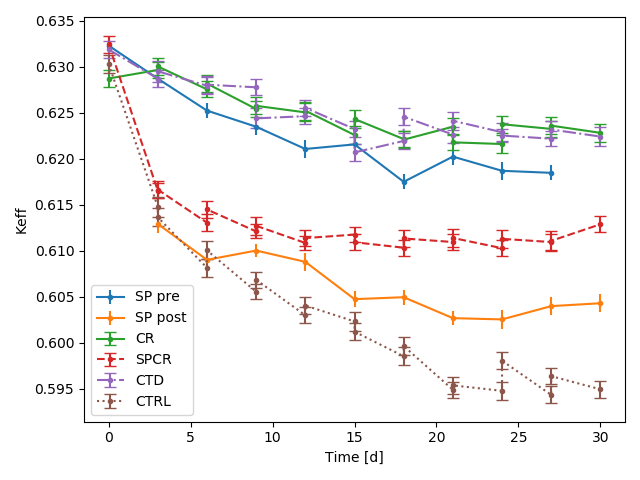
\includegraphics[width=0.45\linewidth]{images/cumulative_keff_batch.png}
%	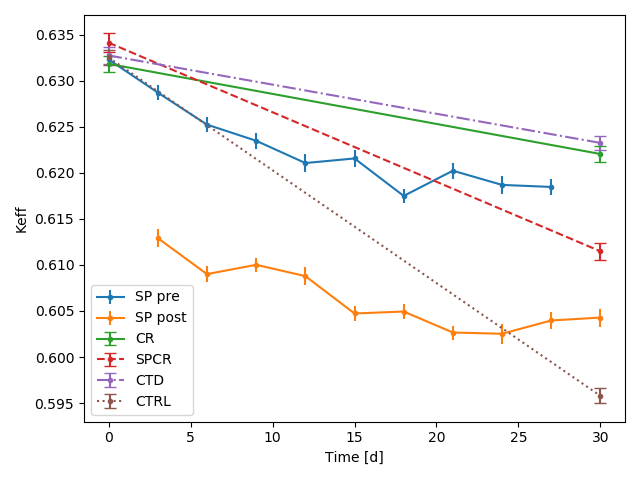
\includegraphics[width=0.45\linewidth]{images/cumulative_keff_coont.png}
%	\caption{Continuous and batch models $k_{eff}$ over time when using the matching depletion steps and feed rates and when continuous uses a single step and average feed rates.}
%\end{figure}

%\begin{itemize}
%	\item \textbf{\emph{SP pre}} is the SaltProc steady batch results pre-depletion (post-reprocessing)
%	\item \textbf{\emph{SP post}} is the SaltProc steady batch results post-depletion (pre-reprocessing)
%	\item \textbf{\emph{CR}} is the Cycle Rate continuous approach
%	\item \textbf{\emph{SPCR}} is the SaltProc Cycle Rate continuous approach
%	\item \textbf{\emph{CTD}} is the Cycle Time Decay continuous approach
%	\item \textbf{\emph{CTRL}} is a control approach with no reprocessing feeds or removal
%\end{itemize}



\textbf{Multiple Steps}
\begin{figure}
	\label{fig:keff_30d_batch}
	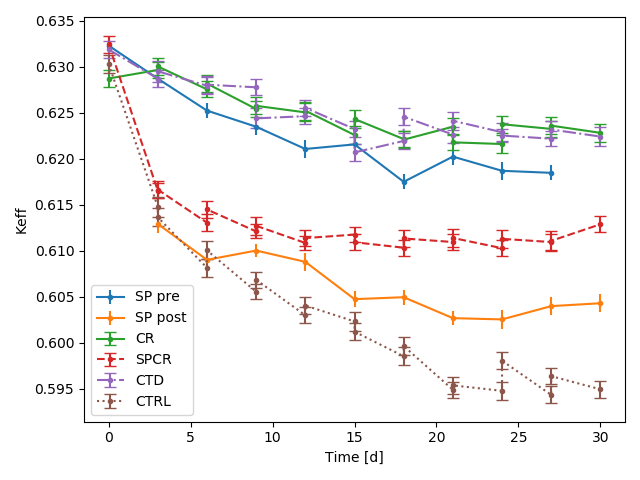
\includegraphics[width=0.9\linewidth]{images/cumulative_keff_batch.png}
	\caption{Continuous and batch models $k_{eff}$ over time when using the matching depletion steps and feed rates.}
\end{figure}

\textbf{Single Step}
\begin{figure}
	\label{fig:keff_30d_batch}
	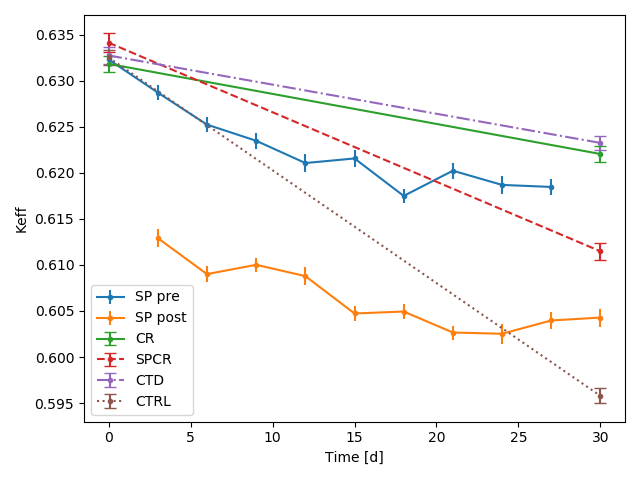
\includegraphics[width=0.9\linewidth]{images/cumulative_keff_coont.png}
	\caption{Continuous and batch models $k_{eff}$ over time when continuous uses a single step and average feed rates.}
\end{figure}


\textbf{Overall Results}

\begin{table}[H]
\renewcommand{\arraystretch}{1.25}
\caption{$k_{eff}$ at 30 Days for 3 and 30 Day Steps}
\label{tab:keff_vals}
%\begin{center}
\begin{tabular}{ | c | c | c | c | }
 \hline
 Approach & 3d Step $k_{eff}$ & 30d Step $k_{eff}$ & Diff [pcm]\\
 \hline
 \hline
 CR & 0.622815 & 0.622043 & 77\\
 SPCR & 0.612871 & 0.611481 & 140\\
 CTD & 0.62241 & 0.623246 & 84\\
 CTRL & 0.594924 & 0.595784 & 86\\

 \hline
\end{tabular}
%\end{center}
\end{table}


\setbeamercolor{block alerted title}{fg=black,bg=norange} % Change the alert block title colors
\setbeamercolor{block alerted body}{fg=black,bg=white} % Change the alert block body colors
\begin{alertblock}{Key Takeaways}
\begin{itemize}
	\item Continuous with same depletion steps results in higher $k_{eff}$
	\item Step size order of magnitude increase and average feed rate usage resulted in ~100 pcm difference in final $k_{eff}$
	\item Step size increase reduces computational cost by a factor of 10
	\item Average feed rate use eliminates double running, making depletion twice as efficient
\end{itemize}
\end{alertblock}

\end{block}



%\setbeamercolor{block alerted title}{fg=black,bg=norange} % Change the alert block title colors
%\setbeamercolor{block alerted body}{fg=black,bg=white} % Change the alert block body colors
%\begin{alertblock}{Future Work }
%\begin{itemize}
%		\item Mass balancing of continuous reprocessing for full reactor
%		\item Comparison of models for full reactor
%		\item Depletion step size development over reactor lifetime
%\end{itemize}
%
%\end{alertblock}

%% This section creates an box with an orange border and a white background
%\setbeamercolor{block alerted title}{fg=black,bg=norange} % Change the alert block title colors
%\setbeamercolor{block alerted body}{fg=black,bg=white} % Change the alert block body colors
%\begin{alertblock}{Future Work }
%\begin{itemize}
%		\item Future work
%\end{itemize}
%
%\end{alertblock}


%----------------------------------------------------------------------------------------
%	ACKNOWLEDGEMENTS
%----------------------------------------------------------------------------------------

\setbeamercolor{block title}{fg=norange,bg=white} % Change the block title color

\begin{block}{Acknowledgements}

	This material is based upon work supported under an Integrated University Program Graduate Fellowship. The authors are grateful for this generous support.

The authors thank Professor Kathryn Huff for her contribution and support of this work in its early stages.
	
\end{block}

%----------------------------------------------------------------------------------------
%	CONTACT INFORMATION
%----------------------------------------------------------------------------------------


\begin{block}{References}

	{\footnotesize\bibliographystyle{abbrv} 
	\bibliography{poster}}
\end{block}


%----------------------------------------------------------------------------------------



\end{column} % End of the third column

\end{columns} % End of all the columns in the poster

\end{frame} % End of the enclosing frame

\end{document}
\begin{column}{\sepwid}\end{column} % Empty spacer column
